\section{测试方案设计}

本章使用功能测试和微基准测试检查三个版本的运行状态。测试对象分别为 main 分支的 C++ + IA32 版本、refactor/x86 分支的 Rust + IA32 版本，以及 refactor/riscv 分支的 Rust + RISC-V 版本。三者均在 QEMU 中运行，测试结论只用于比较本课题关注的内存管理、文件系统和块 I/O 路径，不把结果外推到真实硬件。

测试环境统一控制以下条件：

\begin{enumerate}
  \item QEMU 版本；
  \item 宿主机硬件与操作系统环境；
  \item 虚拟机分配内存大小；
  \item 编译优化选项与编译器版本。
\end{enumerate}

\begin{table}[htbp]
  \centering
  \caption{测试环境说明}
  \begin{tabular}{p{0.20\textwidth}p{0.20\textwidth}p{0.20\textwidth}p{0.20\textwidth}}
    \toprule
    \textbf{测试环境} & \textbf{C++ + IA32} & \textbf{Rust + IA32} & \textbf{Rust + RISC-V} \\
    \midrule
    宿主机操作系统 & Windows 11 专业版 & Windows 11 专业版 & Windows 11 专业版 \\
    QEMU 运行环境 & WSL2 & WSL2 & WSL2 \\
    QEMU 版本 & i386 6.2.0 & i386 6.2.0 & riscv64 10.0.2 \\
    QEMU 分配内存大小 & 128MB & 128MB & 128MB \\
    编译器版本 & g++ 11.4.0 & rustc 1.96.0-nightly & rustc 1.96.0-nightly \\
    编译选项 & 无编译优化 & \texttt{--release} & \texttt{--release} \\
    \bottomrule
  \end{tabular}
\end{table}

性能测试使用仓库 \texttt{programs/} 目录下的三个用户态程序。 \texttt{syscall\_bench.c} 循环执行 open/close、read、seek、stat 和 write，用 \texttt{times()} 记录前后 tick 并换算平均耗时；\texttt{malloc\_bench.c} 对不同大小的内存块重复执行 malloc/free，用于观察用户态动态分配接口在小对象和接近页大小对象上的差异；\texttt{io\_throughput.c} 反复读取源文件并写入目标文件，按总传输字节数估算吞吐率。

需要说明的是，Unix V6++ 的计时来自 60Hz 系统 tick，单个 tick 约为 16.67ms。测试程序把多次循环摊薄为微秒值，但其精度受循环次数、缓存状态和调度时机影响较大。因此，表中数据更适合观察数量级和相对变化，不适合作为硬件级延迟。原始 C++ 版本暂不支持本次 malloc 测试所需的用户态动态分配接口，内存分配部分只比较两个 Rust 版本。

\section{功能测试}

功能测试不追求覆盖所有异常分支，而是先确认系统能否走完课程实验中最常使用的路径。测试内容包括页分配与用户空间增长、文件创建与删除、文件打开与关闭、文件读写、目录创建与路径解析、控制台输入输出，以及 shell 在连续执行命令后的状态保持。测试过程中使用 ls、cat、mkdir、forks 等已有用户程序，并结合新增测试程序检查文件系统和内存分配接口。

从截图和终端输出看，Rust + IA32 版本可以完成原教学系统中的基本文件操作和用户程序执行；Rust + RISC-V 版本可以完成串口初始化、文件系统装载、shell 运行和块设备读写。对本文而言，关键点在于两个 Rust 版本都能够从页分配、文件系统路径解析继续走到块设备读写，说明内存管理和文件系统重构没有破坏系统主路径。

\begin{figure}[htbp]
  \centering
  \begin{subfigure}[b]{0.46\textwidth}
    \centering
    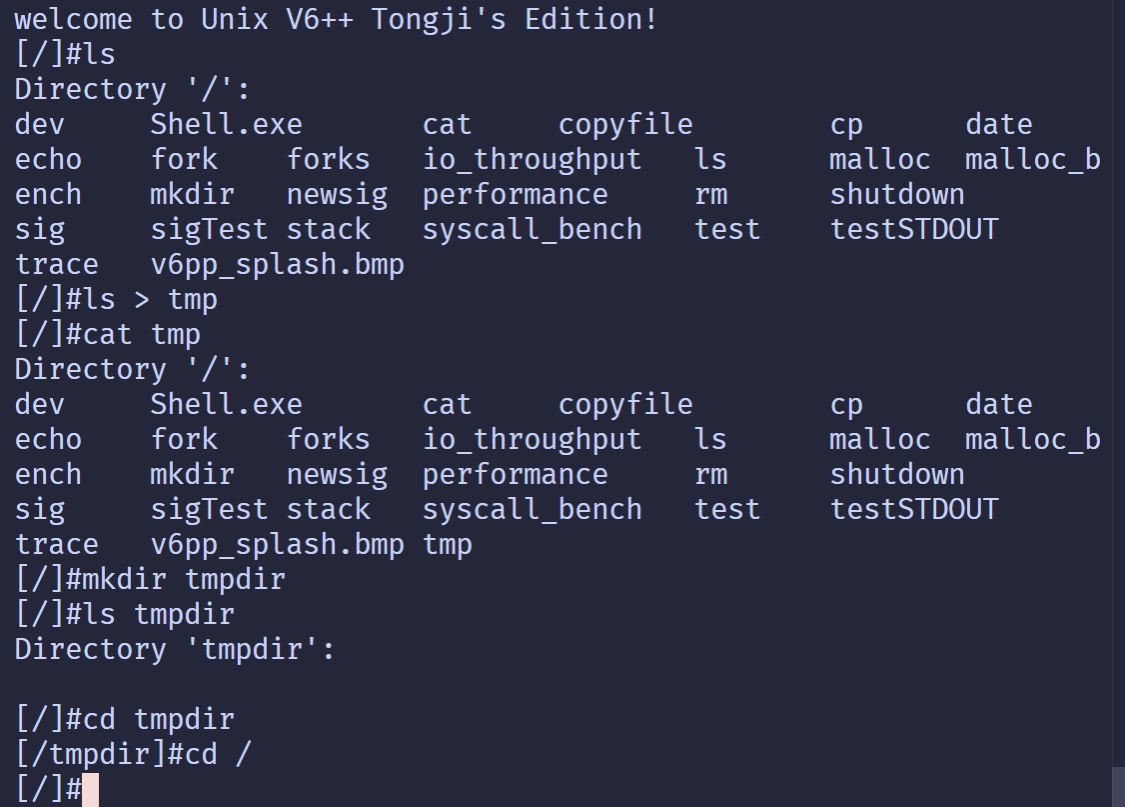
\includegraphics[width=\textwidth]{figures/7/riscv-1.png}
  \end{subfigure}
  \hfill
  \begin{subfigure}[b]{0.46\textwidth}
    \centering
    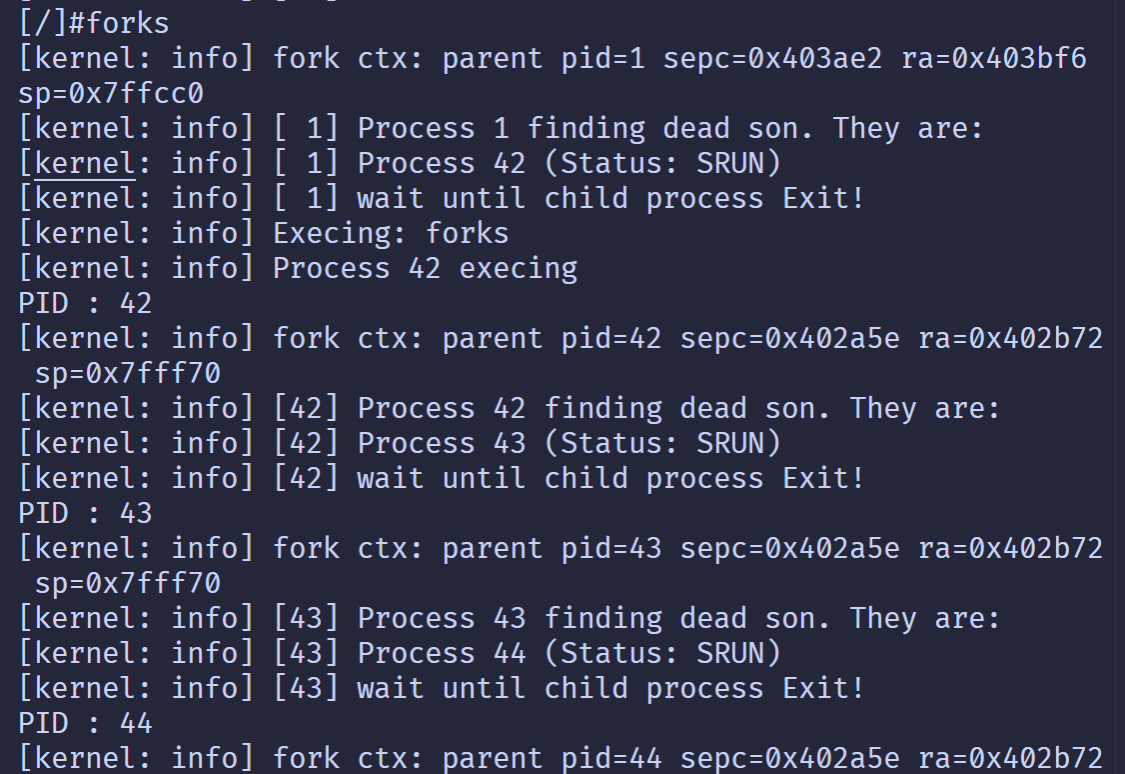
\includegraphics[width=\textwidth]{figures/7/riscv-2.png}
  \end{subfigure}
  \caption{Rust RISC-V 功能测试部分截图}
\end{figure}

\begin{figure}[htbp]
  \centering
  \begin{subfigure}[b]{0.46\textwidth}
    \centering
    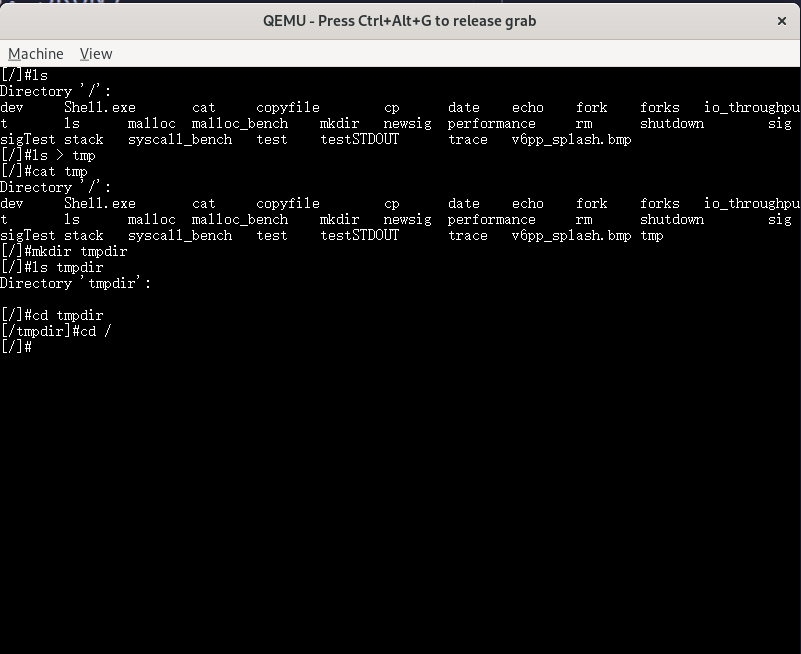
\includegraphics[width=\textwidth]{figures/7/ia32-1.png}
  \end{subfigure}
  \hfill
  \begin{subfigure}[b]{0.46\textwidth}
    \centering
    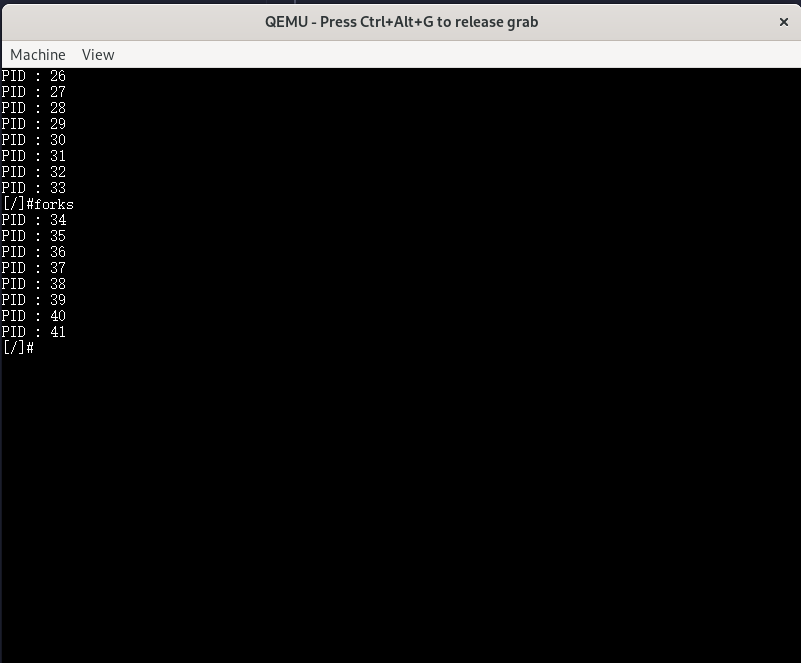
\includegraphics[width=\textwidth]{figures/7/ia32-2.png}
  \end{subfigure}
  \caption{Rust IA32 功能测试部分截图}
\end{figure}

\section{性能测试}

系统调用延迟测试由 \texttt{syscall\_bench.c} 完成。除 write 操作固定执行 5000 次外，其余操作均执行 10000 次；读写缓冲区大小为 512 字节。测试目标文件主要为 \texttt{ls}，write 操作写入临时文件 \texttt{tmp}。由于 open/close、read、stat 与 inode 查找、打开文件表和缓冲区缓存关系较密切，这组测试可作为文件系统主路径开销的近似观察。

\begin{table}[htbp]
  \centering
  \caption{文件系统相关系统调用平均延迟（微秒/次）}\label{tab:syscall-bench}
  \begin{tabular}{p{0.20\textwidth}p{0.20\textwidth}p{0.20\textwidth}p{0.20\textwidth}}
    \toprule
    \textbf{系统调用} & \textbf{C++ + IA32} & \textbf{Rust + IA32} & \textbf{Rust + RISC-V} \\
    \midrule
    open/close & 20 & 8 & 11 \\
    read       & 25 & 6 & 6 \\
    seek       & 1  & 1 & 1 \\
    stat       & 16 & 6 & 8 \\
    write      & 103 & 90 & 106 \\
    \bottomrule
  \end{tabular}
\end{table}

内存分配测试由 \texttt{malloc\_bench.c} 完成。每种块大小下，测试程序每轮分配 20 个对象并释放，重复 50 轮，共执行 1000 次 malloc 和 1000 次 free。原始 C++ 版本暂不支持相同接口，表中以空缺标记。

\begin{table}[htbp]
  \centering
  \caption{用户态 malloc/free 平均延迟（微秒/次）}\label{tab:malloc-bench}
  \begin{tabular}{p{0.20\textwidth}p{0.20\textwidth}p{0.20\textwidth}p{0.20\textwidth}}
    \toprule
    \textbf{分配大小} & \textbf{C++ + IA32} & \textbf{Rust + IA32} & \textbf{Rust + RISC-V} \\
    \midrule
    64B   & -- & 166 & 16 \\
    128B  & -- & 166 & 16 \\
    256B  & -- & 150 & 25 \\
    512B  & -- & 158 & 50 \\
    1KB   & -- & 166 & 83 \\
    2KB   & -- & 166 & 166 \\
    4KB   & -- & 150 & 291 \\
    \bottomrule
  \end{tabular}
\end{table}

文件 I/O 吞吐量测试由 \texttt{io\_throughput.c} 完成。小文件测试以 \texttt{ls} 为源文件，重复复制 5 次；较大文件测试以 \texttt{v6pp\_splash.bmp} 为源文件，复制 1 次。小文件复制容易被缓存命中和 tick 取整放大误差，因此表中对同一版本的多次记录取平均值，只保留可比较的趋势。

\begin{table}[htbp]
  \centering
  \caption{文件 I/O 吞吐量测试结果（KB/s）}\label{tab:io-bench}
  \begin{tabular}{p{0.24\textwidth}p{0.19\textwidth}p{0.19\textwidth}p{0.19\textwidth}}
    \toprule
    \textbf{测试文件} & \textbf{C++ + IA32} & \textbf{Rust + IA32} & \textbf{Rust + RISC-V} \\
    \midrule
    \texttt{ls}，重复 5 次 & 3902 & 2503 & 2691 \\
    \texttt{v6pp\_splash.bmp}，重复 1 次 & 3409 & 4017 & 2556 \\
    \bottomrule
  \end{tabular}
\end{table}

\section{结果分析}

系统调用延迟中，Rust + IA32 在 open/close、read 和 stat 上低于 C++ + IA32。这个差异不宜直接解释为“Rust 更快”，因为三组测试同时改变了代码结构、编译器、编译选项和部分实现细节。更稳妥的解释是，重构后文件对象、inode 引用和错误返回路径被集中整理，open/close 与 stat 中的表项分配、引用计数维护和失败回收更少依赖分散约定。write 的差异较小，说明写路径更多受缓冲区缓存、块设备写回和 QEMU 虚拟设备行为影响。

Rust + RISC-V 在 read、seek、stat 上与 Rust + IA32 接近，open/close 略高，write 接近 C++ + IA32。RISC-V 分支已经替换为 Sv39 页表、trap 入口和 VirtIO MMIO 块设备，而文件系统上层仍沿用同一组 inode、目录项和打开文件表逻辑。由此可以判断，迁移带来的主要差异集中在平台相关路径，文件系统核心算法没有因为架构变化而重写。

内存分配测试呈现出较清楚的大小分界。64B 至 1KB 时，Rust + RISC-V 低于 Rust + IA32；2KB 时二者接近；4KB 时 RISC-V 版本反而更高。小对象通常可以在用户态堆已取得的区域内复用，接近页大小的对象更容易触发页级分配、映射更新或空闲区管理，因此 4KB 一项的开销上升并不意外。这里不能与原始 C++ 版本直接比较，因为该版本没有跑 malloc 测试；但两个 Rust 版本的数据至少说明，RAII 封装和生命周期约束并未妨碍基本动态分配路径工作。

文件 I/O 吞吐量需要谨慎解读。小文件测试中，C++ + IA32 平均值较高，两个 Rust 版本接近；较大位图文件测试中，Rust + IA32 较高，Rust + RISC-V 低于两个 IA32 版本。吞吐量同时受文件系统代码、QEMU 设备模型、缓存命中、块设备驱动、写回策略和 60Hz tick 取整影响。RISC-V 分支使用 VirtIO MMIO 块设备，目前更偏向先打通正确性路径，尚未针对请求合并、中断驱动传输和缓存写回策略做专门优化。

综合三组数据，本文更关注两个结论。其一，Rust 重构后，内存管理和文件系统中引入的类型化接口、RAII 风格封装和显式错误传播没有在测试范围内造成较大的开销；IA32 重构版本在若干文件系统系统调用上还低于原始版本。其二，RISC-V 版本已经能在新的页表、trap 和块设备模型下运行主要功能，但较大文件 I/O 仍受底层设备路径和模拟环境影响，后续优化应优先放在 VirtIO 请求处理和缓存策略上。

\section{本章小结}

本章比较了 C++ + IA32、Rust + IA32 和 Rust + RISC-V 三个版本。功能测试确认两个 Rust 版本均能完成文件系统装载、shell 运行、文件读写和用户程序执行。性能测试覆盖系统调用、malloc/free 和文件复制三类用户态操作。测试结果支持两个判断。内存管理和文件系统的 Rust 重构已经具备可运行性，且没有在主路径上引入明显失控的开销；RISC-V 版本已完成基本迁移，但块设备和 I/O 路径仍是后续性能优化的主要位置。
